\documentclass[twocolumn]{article}

\usepackage{graphicx}
\usepackage{amsmath}
\usepackage{amssymb}
\usepackage{listings}
\usepackage{xcolor}
\usepackage{accsupp}
\usepackage[utf8]{inputenc}
\usepackage{tikz}
\usetikzlibrary{shapes.geometric, arrows.meta, positioning}
\usepackage{pgfplots}
\pgfplotsset{compat=1.18}

%\usepackage[margin=0.75in]{geometry}
\usepackage{authblk}
\usepackage{url}
\usepackage{algorithm}
\usepackage{algpseudocode}
\algblockdefx[EVENT]{Event}{EndEvent}%
  [1]{\textbf{on event}\ \texttt{#1}\ \algorithmicdo}%
  {\algorithmicend\ \textbf{on}}
\algblockdefx[MESSAGE]{Message}{EndMessage}%
  [2][msg]{\textbf{upon message}\ <\texttt{#1}\ |\ #2>\ \algorithmicdo}%
  {\algorithmicend\ \textbf{upon}}
\algnewcommand{\Assert}{\textbf{assert}\xspace}
\MakeRobust{\Call} % for nested Calls


\tikzset{
    block/.style={rectangle, draw, text centered, minimum height=2em, minimum width=5cm},
    triangle/.style={regular polygon, regular polygon sides=3, draw, minimum size=3cm},
    arrow/.style={-{Latex}},
    labelstyle/.style={font=\normalsize},
}

\lstset{
    showstringspaces=false,
    basicstyle=\small\ttfamily,
    numbers=none,
    breaklines=true,
    breakatwhitespace=true,
    columns=fullflexible,
    %breakindent=2ex,
    postbreak=\raisebox{0ex}[0ex][0ex]{\BeginAccSupp{ActualText={}}\ensuremath{\color{gray}\hookrightarrow\space}\EndAccSupp{}},
    tabsize=3
}

\title{Unicity Infrastructure:\\
    the Aggregation Layer}

\author[1]{Risto Laanoja}
\affil[1]{Unicity Labs}

\date{\today}


\begin{document}
\maketitle

\begin{abstract}
Unicity is a new Blockchain Protocol with an ambitious goal---to enable token transactions off-chain, and potentially off-line. There is still some infrastructure needed to e.g. guarantee no double-spending (the \textit{unicity} of spending of every token state). There were no compromises made in building this infrastructure, especially in trust assumptions. This paper focuses on ways the Aggregation Layer---the layer producing the unicity certificates---is built, the efficiency of its design and the strength of the trust and security model.
\end{abstract}


\section{Introduction}

Unicity Network is unique. Its founding idea is to reduce the amount of on-chain data to an absolute minimum. The observation is that shared (``on-chain'') state is unavoidable\footnote{Unless centrally controlled and non-transparent technologies like trusted hardware wallets, TEE-s, etc., are used.} only to avoid double spending. Also, the core tenets are reduced trust requirements, privacy, and no other scaling bottlenecks.


\section{System Architecture}


In order to avoid double-spending of tokens, Unicity Infrastructure permanently\footnote{From the viewpoint of a token, i.e., longer than token lifetime.} remembers a unique identifier of every spent token state. The unique identifier is the hash of the mentioned data. When a user tries to double-spend a token, the identifiers are the same, and it is not possible to fetch another Proof of Unicity from the Unicity Infrastructure. A transaction is void without a bundled Proof of Unicity.

The rest of the processing---executing transactions, running smart contracts, etc.---can happen at the client layer, by so-called ``agents''. Agents are themselves the interested parties of data availability and transaction validation, and choose the ordering of message processing. Thus, the Unicity Infrastructure is relived of these duties, removing the major scaling bottleneck of L1 blockchains.

Unicity Infrastructure operates in a trust-minimized way, by utilizing distributed trusted data structures, and cryptographic SNARKs for extra efficiency. The Proof of Unicity is a fresh \emph{proof of inclusion} of the token state being spent. This can be efficiently generated based on a Merkle Tree data structure. The proof size is logarithmic to the capacity of the tree, thus, efficient. If the tree root is securely fixed, then the rest of the tree is \textit{trustlessly} correct: it is not possible to generate inclusion proofs for anything not in the tree. In fact, the Unicity Infrastructure is a giant distributed Merkle Tree. The infrastructure also supports \textit{non-inclusion proofs}---thus it is possible to prove to other parties that a particular token state is not yet spent. Specifically, the tree is an SMT (Sparse Merkle Tree), or even more specifically, an indexed variant for efficiency reasons. In this paper, we model the distributed tree as an SMT. Furthermore, an SMT is straightforward to shard; we just cut the tree vertically into slices. Leaves are left at their computed positions (SMT is \emph{indexed}); and every leaf's position also encodes its shard address.

The other necessary component for fully trustless operation is a cryptographic proof of consistency, presented to an upstream Consensus Layer to certify every change at the Aggregation layer.

\begin{figure}[!htbp]
    \centering
        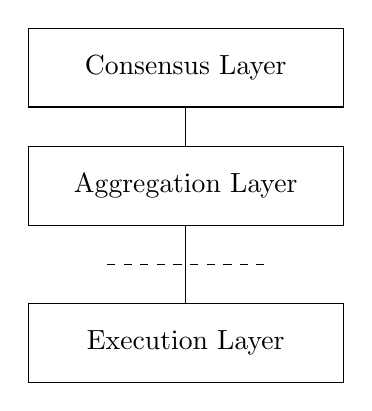
\begin{tikzpicture}
            \draw (0,0) rectangle (4,1) node[midway] {Consensus Layer};
            \draw (2,0) -- (2,-0.5);
            \draw (0,-1.5) rectangle (4,-0.5) node[midway] {Aggregation Layer};
            \draw[dashed] (1,-2) -- (3,-2);
            \draw (2,-1.5) -- (2,-2.5);
            \draw (0,-3.5) rectangle (4,-2.5) node[midway] {Execution Layer};
        \end{tikzpicture}
    \caption{The layered architecture of Unicity Network}\label{fig:layers}
\end{figure}


\subsection{Consensus Layer}

At the root there is a PoW chain, managing the consensus, validators, and the native currency, ALPHA. The chain is quite similar to Bitcoin, the Original Blockchain, and inherits many desirable properties at this layer. By the layers below and some tweaks we avoid most of the less desirable properties.

The PoW layer provides decentralization. Any validator can actively participate in mining, and the blocks are chosen based on the longest chain rule. By picking a PoW mining puzzle that does not yield to speedup by GPUs and specialized hardware (RandomX), we furthermore democratize the participation.

PoW chain's finality is relatively slow and probabilistic. Some rollbacks (``reorgs'') are possible, when alternative chains with stronger PoW appear. At the same time, PoW chains are extremely robust. If any number of validators disappear, or get added, the chain continues growing and the block rate adjusts eventually to the new mining power.

The PoW layer selects validators for the next layer: a BFT finality gadget. A BFT consensus protocol provides finality for underlying layers within seconds, instead of plain PoW's many blocks of ``confirmations'', taking perhaps tens of minutes to accrue enough certainty.

The purpose of BFT consensus is: 1) to provide deterministic (one-block) finality for layers below, 2) achieve a fast and predictable block rate. On the other hand, BFT consensus is more fragile because the liveness of BFT consensus depends on the availability of a certain ratio of honest validators.

The usual way to achieve \emph{permissionless} BFT consensus is to use a Proof of Stake (PoS) setup. This is fragile, especially during the bootstrapping of a blockchain protocol. PoW (longest-chain-rule based protocols in general) are more robust and great to achieve initial token distribution and value for effective decentralization.

By combining a PoW chain with an underlying BFT consensus layer, Unicity provides good properties of both approaches to the layers below. The PoW chain provides decentralization and robustness, and high security of the base currency (as the asset); BFT provides determinism, speed and finality.

BFT consensus is like a \emph{finality gadget}, but with a much higher block rate. BFT validators are selected based on PoW layer validator performance: recent successful and well-behaving PoW miners are becoming (or can delegate) BFT Consensus Layer validators.

Consensus Layer validators get their block rewards after the end of every epoch. It is possible to increase economic security by implementing slashing based on withheld PoW layer and Consensus layer block rewards.

Introduction of economic security is a part of evolving the Consensus Layer to Proof of Stake consensus. This would provide maximal economic security for the BFT nodes, and be more efficient and environmentally responsible than PoW mining.

\subsection{Aggregation Layer}

The Aggregation (Unicity, SMT) layer implements a global, immutable key-value store which marks all spent transactions as spent, forever. It is possible to obtain a compact cryptographic certificate of a state being spent. The value part of the key-value tuple ties the certificate to an input state (transaction).

\begin{figure*}[!t]
    \centering
    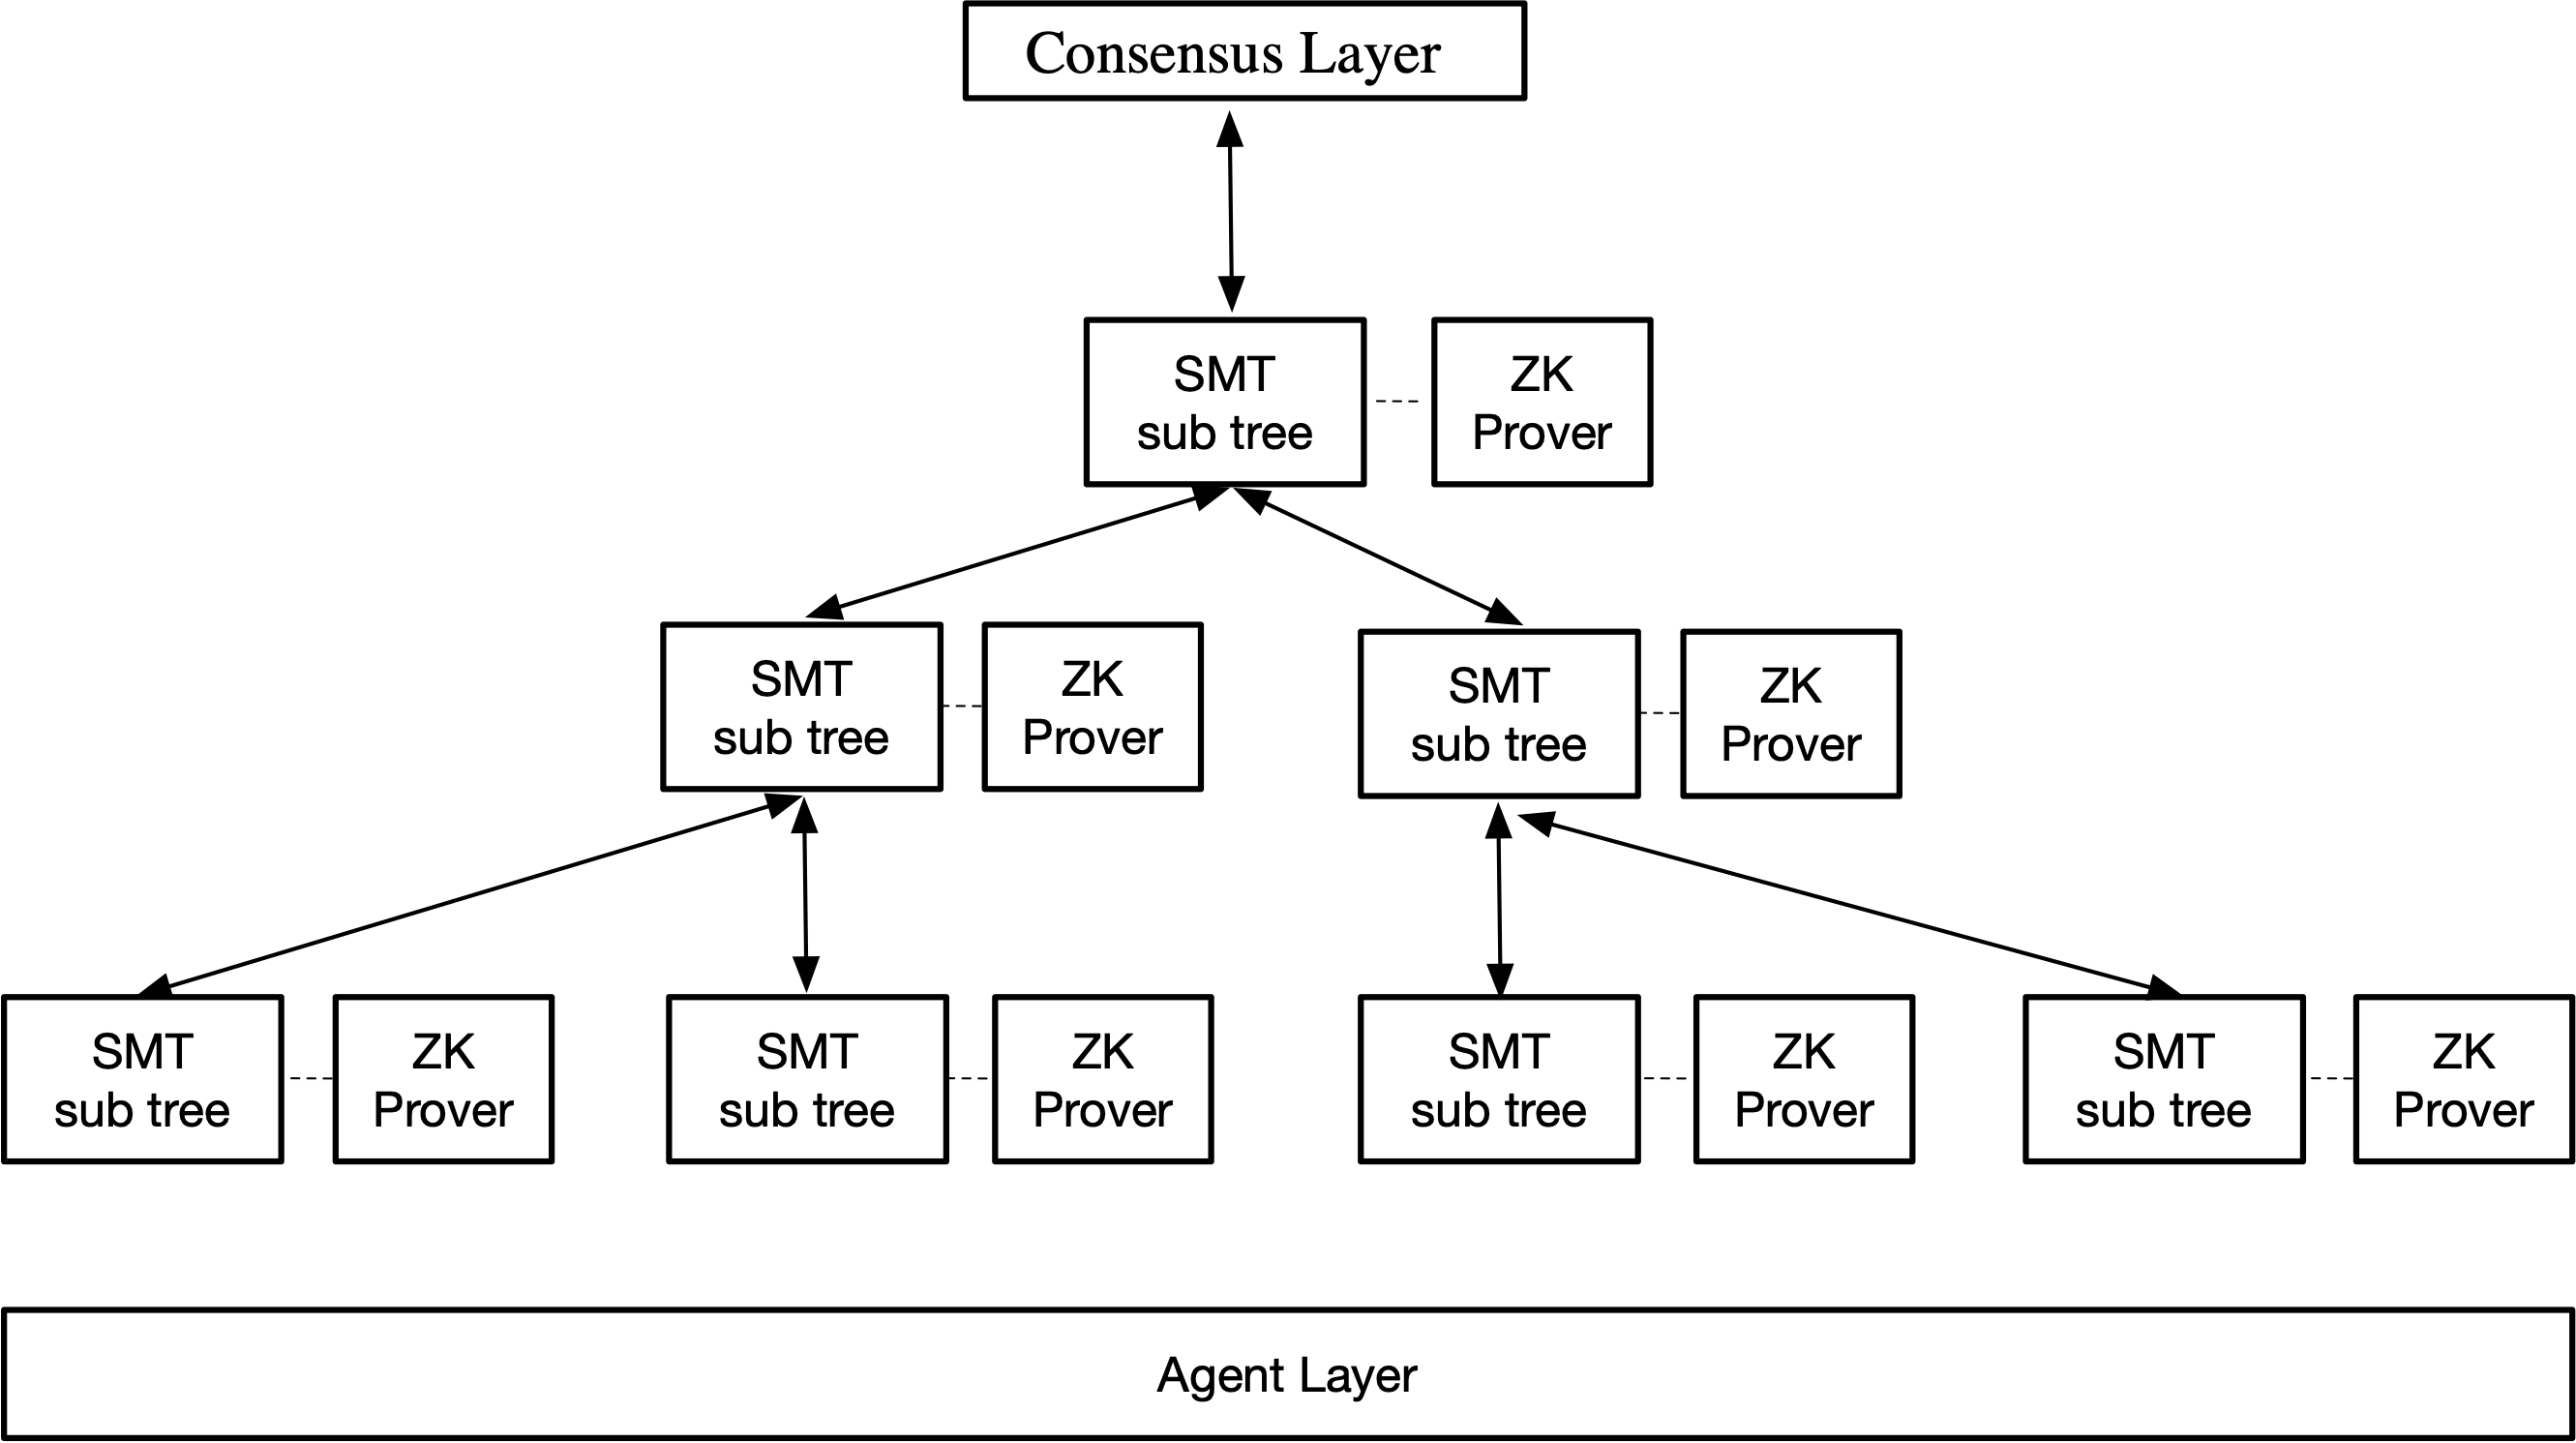
\includegraphics[width=.7\textwidth]{pic/layers}
    \caption{The sharded architecture of Aggregation Layer}\label{fig:sharding}
\end{figure*}

The Aggregation layer is sharded based on keyspace slices, and can be made hierarchical: see Fig.~\ref{fig:layers}.

\emph{Proof of non-deletion}: once a leaf is set, it is there \emph{relatively} forever; and every state change of the SMT or slice of the SMT is accomplished with a cryptographic proof of pre-existing leaves being the same. The proof size is logarithmic to the capacity plus linear to the inclusion batch size. This can be reduced to a constant size by a SNARK.

\subsection{Execution Layer}

The Agent Layer is executing transactions and other business logic, consuming the services of the Aggregation Layer.


\section{Aggregation Layer}

A trustless append only accumulator is \emph{consistent}, if during the insertion of a batch of updates there were no changes or deletions of existing leaves. The data structure implements other usual functions like inclusion proofs and non-inclusion proofs.

The size of the consistency proof depends on the size of the addition batch and the logarithm of capacity. If we denote batch size as $k$ and depth $d$, then the size of the consistency proof is $O(k \cdot d)$, where $d \approx \log(capacity)$.

By using a cryptographic SNARK (a zero knowledge proof with certain properties), the size of the consistency proof can be further reduced to a constant size.

After every addition batch, the root of the aggregation layer is certified by the BFT Finality Gadget, ensuring its uniqueness and immutability. This provides a useful trust anchor for consistency proofs, inclusion proofs, and non-inclusion proofs.


\subsection{Security Model}

The Aggregation Layer implements an append-only authenticated dictionary data structure.

\begin{figure}[!htbp]
    \centering
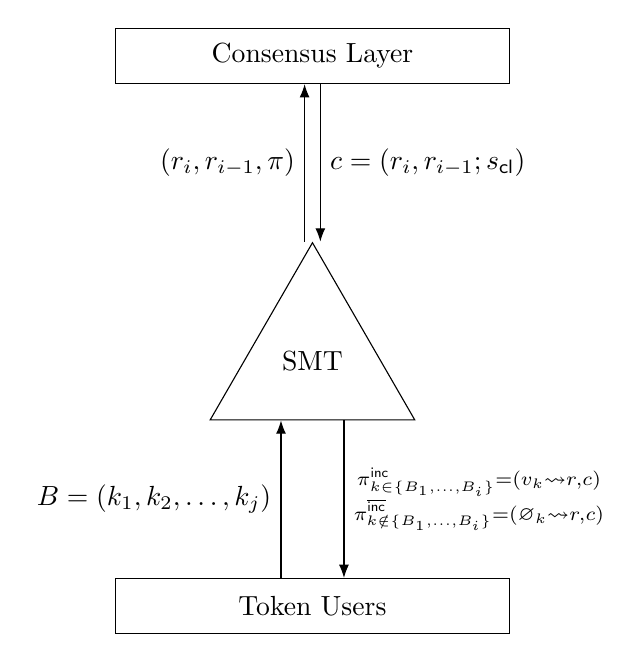
\begin{tikzpicture}[node distance=2cm and 2cm]

    % Nodes
    \node[block] (consensus) {Consensus Layer};
    %\node[block, below=of consensus] (triangle) {}; % dummy node for triangle placement
    \node[triangle, below=of consensus] (triangle) {SMT};
    \node[block, below=of triangle] (users) {Token Users};

    % Arrows
    \draw[arrow] ([xshift=-0.1cm]triangle.north) -- ++(0,1) node[labelstyle, left] {$(r_i, r_{i-1}, \pi)$} -- ([xshift=-0.1cm]consensus.south);
    \draw[arrow] ([xshift=0.1cm]consensus.south) -- node[labelstyle, right] {$c = (r_i, r_{i-1}; s_{\textsf{cl}})$} ([xshift=0.1cm]triangle.north);
    \draw[arrow] ([xshift=-0.4cm]users.north) -- node[labelstyle, left] {$B = (k_1, k_2, \ldots, k_j)$} ([xshift=-0.4cm]triangle.south);
    \draw[arrow] ([xshift=0.4cm]triangle.south) -- ++(0,-1) node[labelstyle, right] {
            $\substack{
                \pi^{\textsf{inc}}_{k \in \{B_1, \dots, B_i\}} = (v_k \leadsto r, c) \\
                \pi^{\overline{\textsf {inc}}}_{k \notin \{B_1, \dots, B_i\}} = (\varnothing_k \leadsto r, c)
            }$
            } -- ([xshift=0.4cm]users.north);

\end{tikzpicture}
    \caption{The Security Model of Aggregation Layer}\label{fig:model}
\end{figure}

It authenticates incoming state transfer certification requests by verifying if the sender is in possession of the private key of the key-pair the current token owner is identified with. Specific protocol details are out of scope of this paper.

Authenticated requests are processed by batches $B_i$. At the end of each batch, the Aggregation Layer produces its summary root hash $r_i$ and sends it to the Consensus Layer for certification. A certification request $(r_i, r_{i-1}, \pi)$ includes: 1) previous state root hash, 2) new state root hash, 3) consistency proof of the changes made during the batch, 4) authenticator identifying the operator.

Consensus layer certifies the request only if it uniquely \textit{extends} a previous non-certified state root hash, and the consistency proof is valid. It returns a certificate $c = (r_i, r_{i-1}; s_{\textsf{cl}})$, where $s_{\textsf{cl}}$ is the signature of the Consensus Layer (group signature of the consensus nodes, or proof of inclusion in a block).

One state can be extended only once---this guarantees that the entire aggregation layer is not forked.

The next round extends the newly certified state, and so on.

We model the Consensus Layer as an oracle, see Algorithm~\ref{alg:consensuslayer}.

\begin{algorithm}[tbh]
  \caption{Consensus Layer modeled as an oracle}\label{alg:consensuslayer}
  \begin{algorithmic}[0]
    \Function{Initialize}{\null}
        \State $r_- \gets \bot$
        \State $i \gets 0$
    \EndFunction
    \Function{CertificationRequest}{$(r_i, r_{i-1}, \pi)$}
        \If {$(r_{i-1} \ne  r_-) \lor \lnot\Call{valid}{\pi, r_i, r_{i-1}}$}
            \State \Return $\bot$
        \EndIf
        \State $r_- \gets r_i$
        \State $i \gets i+1$
        \State $s_{\textsf{cl}} \gets \textsf{sig}_\textsf{cl}(i, r_i, r_{i-1})$
        \State \Return $c = (i, r_i, r_{i-1}; s_{\textsf{cl}})$
    \EndFunction
  \end{algorithmic}
\end{algorithm}


SMT can return trustless inclusion and non-inclusion proofs to the user; where each proof is certified by a certificate from the Consensus Layer.

The Consensus layer must guarantee its data availability---otherwise, if e.g. some last states are lost, then it is not possible to generate a valid state transfer request, and also last certified hashes could be double-spent by malicious users. Therefore, it is necessary to provide a redundant service. It is not necessary to have a consensus at this layer. Running a protocol like Raft is perfectly good and efficient.

The Aggregation layer must not modify its registered state hashes and not remove any previously stored state hashes. If a cryptographic proof of non-deletion and non-modification (see Section~\ref{sec:consistency-proof} below) is included in a certification request, then the Aggregation Layer is \emph{trustless}.


\section{Consistency Proof}
\label{sec:consistency-proof}

A Consistency Proof is a data structure proving the consistency of one round of operation of the Append Only Accumulator.

We have the $i$-th batch of insertions $B = (k_1, k_2, \dots, k_j)$, where $k$ is an inserted item; all insertions are executed during a round of operation. The root hash before the round is $r_{i-1}$, and after the round is $r_i$. The accumulator is implemented as a Sparse Merkle Tree (SMT).

The consistency proof generation for batch $B_i$ works as follows:

\begin{enumerate}
    \item Insert the new SMT leaves in $B_i$.
    \item Starting from the newly inserted leaves, for each sibling hash necessary to compute the root of the tree, we record the sibling's path and the sibling's value as the proof. Let's denote the set as $s_i$.
    \item Record $(B_i, r_{i-1}, r_i, s_i)$.
\end{enumerate}

Proof verification works as follows:

\begin{enumerate}
    \item Authenticate $r_{i-1}, r_i$.
    \item Build an incomplete SMT tree: for each item in $B_i$, we insert the value of an empty leaf at the appropriate position.
    \item All necessary siblings necessary to compute the root are available in $s_i$. Compute the root, compare with $r_{i-1}$; if not equal then the proof is not valid.
    \item Build again an incomplete SMT tree; for each item in $B_i$, we insert the value of each key into the appropriate position.
    \item Compute the root based on siblings in $s_i$. If the root is not equal to $r_i$ then the proof is not valid.
    \item The proof is valid if the checks above passed.
\end{enumerate}

This shows that given authentic $r_{i-1}, r_i$, the keys in $B_i$ were empty before the insertion batch, and after execution of the insertion batch the values in $B_i$ were recorded at the positions defined by their respective keys, and there were no other changes.

\begin{algorithm}[tb]
  \caption{Verification of non-deletion proof}\label{alg:verifynondeletion}
  \begin{algorithmic}[0]
    \Function{VerifyNonDeletion}{$\pi, r_{i-1}, r_i, K, V$}
      \State   \Comment{Proof $\pi$ is an array of dictionaries}
      \State   \Comment{Assumes that keys in $K$ are sorted}
      \State $p_\varnothing \gets \{(k, \varnothing) \mid k \in K\}$ \Comment{empty leaves}
      \State $r_\varnothing \gets$ \Call{ComputeForest}{$\pi, p_\varnothing$}
      \State \textbf{assert} $r_\varnothing = r_{i-1}$
      \State \Comment{Same with batch's leaves populated}
      \State $p_B \gets \{(k, v) \mid (k,v) \in (K, V)\}$
      \State $r_B \gets$ \Call{ComputeForest}{$\pi, p_B$}
      \State \textbf{assert} $r_B = r_i$
      \State \Return $1$ \Comment{Success}
    \EndFunction

    \Function{ComputeForest}{$\pi, p$}
      \For{$\ell \gets \text{tree\_depth}-1 \textbf{ to } 0$}
        \State $p' \gets [\,]$
        \State $i \gets 0$
        \While{$i < |p|$}
          \State $(k, v) \gets p[i]$
          \State $k_p \gets \lfloor k / 2 \rfloor$ \Comment{Parent key}
          \State $\text{is\_right} \gets k \bmod 2$
          \State $k_s \gets 2k_p + (1 - \text{is\_right})$ \Comment{Sibling key}
          \If{$\lnot \text{is\_right} \land |p| > i+1 \land p[i+1].k = k_s$\\ \hskip 4em}
                                         \Comment{Special case: }
            \State $v_s \gets p[i+1].v$  \Comment{right sibling is next}
            \State $i \gets i + 1$       \Comment{jump over.}
          \Else                          \Comment{Get sibling value from proof,}
            \State                       \Comment{assign $\varnothing$ if not in layer's dict}
            \State $v_s \gets \pi[\ell].\text{get}(k_s).\text{or\_else}( \varnothing)$
          \EndIf
          \State $v_p \gets h(v_s, v)$ \textbf{if} is\_right \textbf{else} $h(v, v_s)$
          \State $p' \gets p' \cup (k_p, v_p)$
          \State $i \gets i + 1$
        \EndWhile
        \State $p \gets p'$
      \EndFor
      \State \textbf{assert} $|p| = 1$ \Comment{One root!}
      \State \Return $p[0].v$ \Comment{Value of the root}
    \EndFunction
  \end{algorithmic}
\end{algorithm}


\section{(ZK)-SNARKs}

By using an appropriate cryptographic SNARK, the size of the consistency proof can be reduced to a constant size. Proof generation time depends on the logarithm of capacity and the max. addition batch size.

The statement to be proved is the verification algorithm sketched above. The instance is defined by the root of trust and insertions, $I = ((r_i, r_{i-1}),B_i)$. The witness $\omega = (s_i)$ is the secret in zero knowledge, but for our use-case, it is not necessary to keep the witness secret.

The statement is implemented as a constraint system $R$ using the CIRCOM domain specific language. The witness is generated based on $s_i, B_i$, and supplemented by control wires defining how individual hashing blocks in the circuit are connected to the previous layer and to the inputs. If all constraints are satisfied, then the proof is valid.

The proving backend is Groth 2016\footnote{\url{https://eprint.iacr.org/2016/260}} with a conveniently small proof size. The proving time depends on the depth of the SMT and the maximum size of the insertion batch. Importantly, the proving effort does not depend on the total size/capacity of the SMT, enabling fairly large instantiations.

If the layer above verifies proofs of consistency, then the Unicity aggregation layer is trustless. Still, some redundancy (at least one node able to persist the data structure) is required for data availability.


\section{Circuit-based SNARK definition}

Due to the limited expressivity of an arithmetic circuit---there are no loops, no recursion, no (literal) branching---the computation is executed from top to bottom as the circuit is computed, it helps to first pre-process the inputs.

We add a ``wiring'' signal to the circuit, which is a pre-computed part of the witness. This signal defines how the inputs are connected to the hashing blocks in the circuit.

Preprocess the proof:

\begin{enumerate}
    \item Flatten the SMT (hash forest containing proof + addition batch) to the left (root is up),
    \item sort by layers, leaves first, and then lexicographically,
    \item add a 'wiring' signal fed into MUXes in the inputs of each hasher cell.
\end{enumerate}

Let's denote maximum batch size $k_{max}$, SMT depth $d$. Because the circuit is statically generated, it must be sized based on the largest batch it is able to process.

The circuit has two halves, both controlled by the same wiring signal. Note that it is also critical to security that the control signal and proof are the same for both halves. The first half connects all insertion batch indices to zero (the value of an empty element), the second half to the actual input values of the batch.
The first half computes to the root hash before the insertion batch. The second half---after.

The size of each half is $k_{max} \cdot d$.

Every following hashing layer connects inputs either to an output from the previous layer, or an element from the proof.

The wiring signal is a pre-computed part of the witness and does not have to be public. This is a lot of wires; let's see the effect on proving time.

\begin{figure*}[!t]
    \centering
    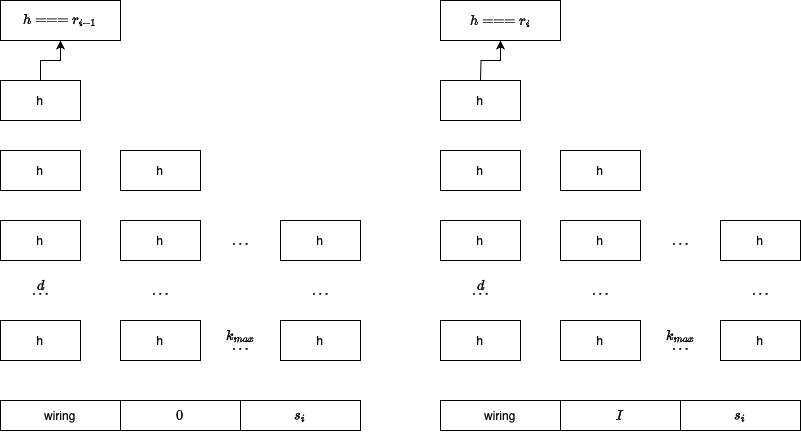
\includegraphics[width=0.9\textwidth]{pic/smt-circuit.drawio}
    \caption{Circuit structure}\label{fi:smt-circuit}
\end{figure*}

Each cell above is implemented as a template with 2 MUXes and a 2:1 hasher:

\begin{figure}[t]
    \centering
    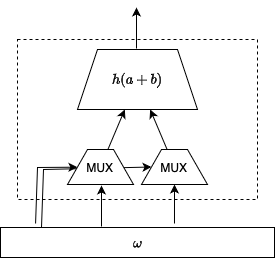
\includegraphics[width=.6\columnwidth]{pic/smt-circuit-cell.drawio}
    \caption{One hashing cell of the circuit}\label{fi:smt-circuit-cell}
\end{figure}


The leaf layer, first half MUX inputs are connected to a vector with:
\begin{itemize}
    \item `empty' leaf ($0$)
    \item all the new leaves in the batch are connected to `empty' ($0$)
    \item `proof' or sibling hashes ($s_i$)
\end{itemize}

The leaf layer, second half MUX inputs are connected to a vector with:
\begin{itemize}
    \item `empty' leaf ($0$)
    \item batch of new leaves ($I$)
    \item identical `proof' or sibling hashes ($s_i$)
\end{itemize}

Internal layers' MUXes are connected to a vector with:
\begin{itemize}
    \item `empty' leaf ($0$)
    \item previous layer cell output hashes,
    \item `proof' or sibling hashes ($s_i$)
\end{itemize}

Both halves' MUXes are controlled by the same wiring signal. The positions of batch elements and proof elements are encoded into the control wires during the pre-processing, that is, control signals are part of the witness.

\subsection{Performance Indication}

On a consumer laptop (Macbook M1), the proving throughput, using the Poseidon hash algorithm, is up to 25 tx/s.

\section{Execution Trace-based STARK}

We have a fixed circuit written as a Rust program. As a commitment to the ``right'' verification program we use a prover key, generated during setup. Its contents are: a commitment to the preprocessed traces, the starting Program Counter register, the starting global digest of the program, after incorporating the initial memory; the chip information, the chip ordering. Probably prover config -- underlying finite field, PCS scheme, etc. -- as well.

For verification, we obtain the prover key hash and authenticate it off-band.

\begin{sloppypar}
After verifying the proof (\lstinline|client.verify(&proof, &vk)|), we can be sure that \lstinline|proof: SP1ProofWithPublicValues| is valid. The proof data structure embeds its validated ``instance'', or public parameters. Based on these parameters we check that indeed, the right thing was validated by our program. In our case the instance is defined by the old root hash, new root hash, and the batch size. Now we know, that the proof (this is the hash-based non-deletion proof of the SMT's change being consistent) verification algorithm was executed correctly, and this algorithm was happy with its public and private inputs; and thereby the batch of additions inserted into the SMT was also executed correctly: started its processing with an initial state and after inserting n transactions (and not removing nor modifying any existing leaves) reached the final summary state. Obviously, the before-state and after-state must be authentic. This is achieved by committing them to an append-only dictionary / blockchain / Unicity's BFT layer.
\end{sloppypar}

We do not care about the privacy of the ``secret'' witness. Not sure if used STARKs implementations provide it neither. So, no zk in zk-SNARKs, just proof of computational integrity.


\subsection{Optimization Ideas}

The elephant is the underlying hashing function.

At the time of writing, SP1 zkVM\footnote{\url{https://docs.succinct.xyz/docs/sp1/introduction}} has precompiles for SHA2 and SHA3/Keccak, so these are somewhat accelerated. See program output -- which precompiles (aka coprocessors, chips) are used and how many times, e.g., \lstinline|... SHA_EXTEND: 3552, SHA_COMPRESS: 3552, ...|. We're using SHA2-256, which is rather slow to prove!

A possible optimization is the use of specific ``ZK friendly'' hash functions. It works great on circuit based arithmetization with direct access to computational units, or (finite) 'field elements'. On RISC-V zkVM's it is nuanced. A program sees only 32-bit CPU registers; to overcome it, there are some precompiles which are implemented as circuits -- thus can provide some benefit; but there is still a translation expense between 32-bit integer registers and native field elements. Range checking to detect overflows is not efficient in ZK! There are attempts with ZK friendly hash function precompiles\footnote{\url{https://github.com/Okm165/sp1-poseidon2/pull/8}}, with limited real-world effect.


\subsection{More on ZK and Hash Functions}

Standardized cryptographic hash algorithms are optimized for the minimal physical chip area. This is NIST's choice. Some others for fast execution on CPU, like the Blake family. They all include lots of operations which are easy on silicon logic like rotations, bitwise operations, etc. These are notoriously slow for ZK provers though. Usually, one bit is represented as a full field element (for example, on a BN254 field -- a whole 254 bit value per one bit!\footnote{See e.g. \url{https://github.com/iden3/circomlib/blob/master/circuits/sha256/sha256.circom}}). Also, ZK likes linear operations like +, -, and multiplication. The rest is emulated through those.

There are some newer cryptographic hash functions specifically designed for ZK efficiency in mind, like Poseidon, Poseidon2, which are already somewhat established but still young; some are better on large fields (Reinforced Concrete), some on smaller (Monolith), while depending on the proof system's lookup table support. Some are bleeding edge (Griffin, Anemoi) and super fast. Some are even okay-ish on a silicon CPU, e.g., GMiMC.

These operate on full field elements without translation. Security level is defined by the underlying field and instantiation parameters. The smaller the field, the more field elements we need for the hash function's state and output. But still, only a few.

Different zkVM's have different sets of precompiles. Basically all run on RISC-V 32-bit integers. Cairo / Starknet VM provides direct access to the field elements , but its VM is rather specialized to be used for a L2 roll-up.


\subsection{Performance Indication}

On a consumer laptop (10-core Macbook M1), the proving time of a 500-transaction batch, using the SHA2 hash function, is 5 minutes. But, SP1 goes like a bulldozer, whatever one throws at it. It supports distributed prover networks and industrial-grade GPUs and proof recursion and whatnot.


\subsection{How to avoid the bottleneck}

The setup is quite optimal: proving time depends on the size of the addition batch (NOT batch size times tree capacity). The verification algorithm looks tight.

We need to use ZK friendly hash functions. The framework should provide direct access to native field elements, as used by the arithmetization layer (this excludes zkVMs). The execution trace generation must be super fast (this excludes Cairo 0). The prover must be fast; state of the art is small fields (BabyBear, Mersenne 31 etc), and a prover based on FRI, and Circle-STARK: candidates are Plonky3\footnote{\url{https://github.com/Plonky3/Plonky3}} and STwo\footnote{\url{https://github.com/starkware-libs/stwo}}. Better if reasonably mature and modular and open. Leaving us with Plonky3.

And the verification algorithm must be hand-crafted as a custom AIR circuit.

\subsection{Performance Indication}

Indirect test with similar computation (Plonky3 framework, Poseidon2 hash function, small Koala Bear finite field) shows the expected proving performance of this stack being 10000 tx/s, on a 10-core CPU, blowup factor $2^1$, proof size 1.7 MB, or with a less aggressive configuration with blowup factor $2^3$ approx 2500 tx/s, with proof size 670 kB, and increased prover memory requirement.

This shows that running the Aggregation Layer trustlessly is economically quite feasible.

We note that the Poseidon family of hash functions is rather new and has seen much less cryptographic analysis than traditional hash functions like SHA2, Blake family; but amongst the new wave of ZK-friendly arithmetic hash functions, it has seen most of the scrutiny and can be tentatively considered as secure. On the other hand, we win about $50x$ in proving effort compared to, e.g., Blake 3.


\subsection{Summary}

Zero knowledge proofs are a great way to compress the size of consistency proofs. For different use-cases and parameters different tools are optimal. For very small addition batches, just a hash-based proof, whose size is linear to the batch size, is optimal. But when the batch is larger or bandwidth is limited then ZK compression becomes useful.

Some of the proof systems produce larger proofs at the cost of reduced proving complexity and generality, i.e. lack of a trusted setup; some produce very small proofs at the cost of proof effort, a trusted setup which may be circuit specific.

For more complicated use-cases a hybrid setup and proof recursion are useful. See Fig.~\ref{fig:comp} for how previously discussed technologies compare.

\begin{figure}[!htbp]
    \centering
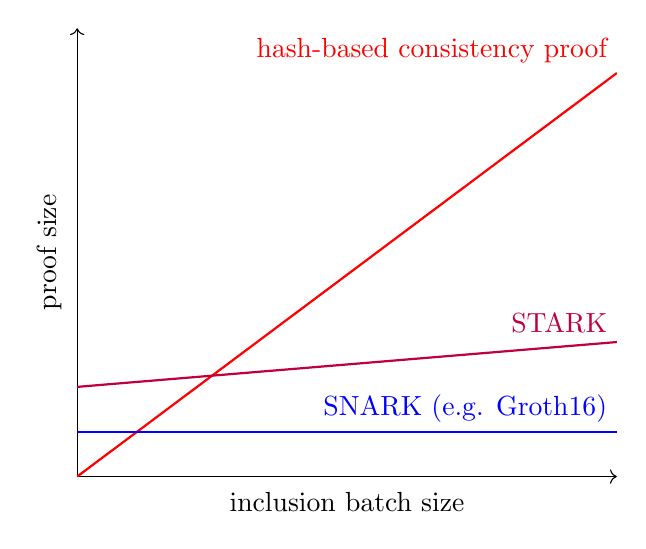
\begin{tikzpicture}
\begin{axis}[
axis lines = left,
axis line style={->},
xlabel = {inclusion batch size},
ylabel = {proof size},
xmin=0, xmax=10,
ymin=0, ymax=10,
xtick=\empty,
ytick=\empty,
]
\addplot [red, thick, smooth] coordinates {(0,0)  (10,9)};
\node [red, above left] at (axis cs:10,9) {hash-based  consistency proof};

\addplot [purple, thick, smooth] coordinates {(0,2) (10,3)};
\node [purple, above left] at (axis cs:10,3) {STARK};

\addplot [blue, thick, smooth] coordinates {(0,1) (10,1)};
\node [blue, above left] at (axis cs:10,1) {SNARK (e.g. Groth16)};
\end{axis}
\end{tikzpicture}
    \caption{Proof size vs. use of ZK compression. Note that while STARKs produce generally larger proofs, they're easier to compute and do not depend on a trusted setup.}\label{fig:comp}
\end{figure}


\begin{thebibliography}{9}

\bibitem{wp} The Unicity Developers: Unicity Whitepaper (2025) \url{https://github.com/unicitynetwork/whitepaper-tex/releases/tag/latest}

\bibitem{snark} Trustless SMT accumulator \url{https://github.com/unicitynetwork/nd-smt}

\bibitem{stark} SP1 zkVM based consistency proof \url{https://github.com/unicitynetwork/zkvm-ndsmt}

\end{thebibliography}

\end{document}
